\section{Câu 12}
Cho mạch điện như ở Hình 7a. OPAMP được cấp nguồn có $V_{OH}=3.3V$, $V_{OL}=-3V$.
Các điện trở được chọn $R_1=2K$, $R_2=5K$, $R_3=4K$.\\
Cho dạng sóng Vi(t) như ở Hình 7b. Vẽ dạng sóng ngõ ra Vo trong các trường hợp sau:\\
a. $V_1=2V$, $V_{m1}=2V$, $V_{m2}=-3V$\\
b. $V_1=4V$, $V_{m1}=1V$, $V_{m2}=-3V$
\begin{figure}[H]
	\centering
	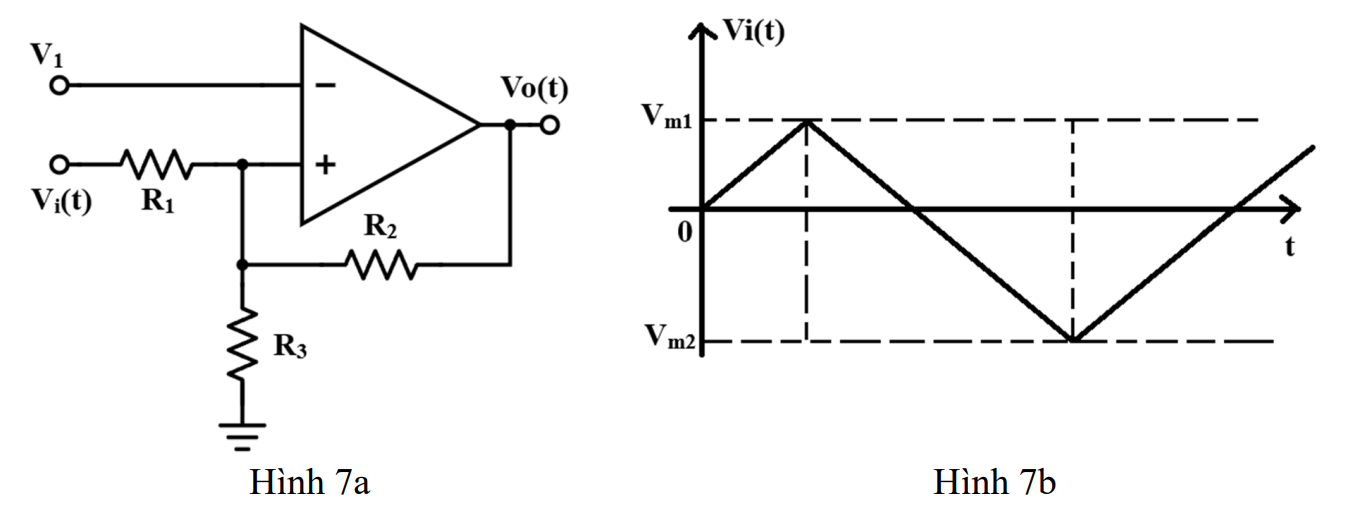
\includegraphics[scale=0.6]{image/C12_De.png}
\end{figure}
\begin{center}
\textbf{Bài giải}
\end{center}
a. Giả sử OPAMP lý tưởng:\\
Ta có:
\[
\left\{
\begin{aligned}
V^- &= V_1 \\
V^+ &= \dfrac{\dfrac{V_i}{R_1} + \dfrac{V_0}{R_2}}{\dfrac{1}{R_1} + \dfrac{1}{R_2} + \dfrac{1}{R_3}} = \dfrac{10}{19}V_i +\dfrac{4}{19}V_o
\end{aligned}
\right.
\]

\[
\begin{aligned}
&\text{Giả sử }& V_o = V_{OH} &\qquad\rightarrow\qquad V^+ = \dfrac{10}{19}V_i + \dfrac{4}{19}\cdot3.3 \quad;\quad V^- = 2 \\
&\text{Để }& V_o = V_{OL} &\qquad\rightarrow\qquad V^+ < V^- \quad\rightarrow\quad \boxed{V_i<2.48V}\\
&\rightarrow& V_o = V_{OL} &\qquad\rightarrow\qquad V^+ = \dfrac{10}{19}V_i + \dfrac{4}{19}\cdot-3 \quad;\quad V^- = 2 \\
&\text{Để }& V_o = V_{OH} &\qquad\rightarrow\qquad V^+ > V^- \quad\rightarrow\quad \boxed{V_i>5V}\\
\end{aligned}
\]\\
Vì $V_i<2.48V \rightarrow V_o$ luôn bằng $V_{OL}=-3V$ 
\begin{figure}[H]
	\centering
	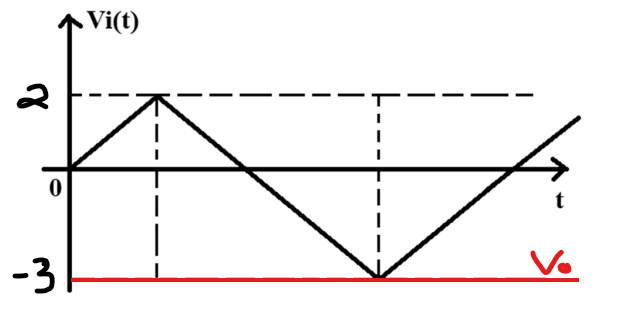
\includegraphics[scale=0.6]{image/C12_a_BT.png}
\end{figure}

\begin{figure}[H]
    \centering
    \begin{subfigure}[b]{0.48\textwidth}
        \centering
        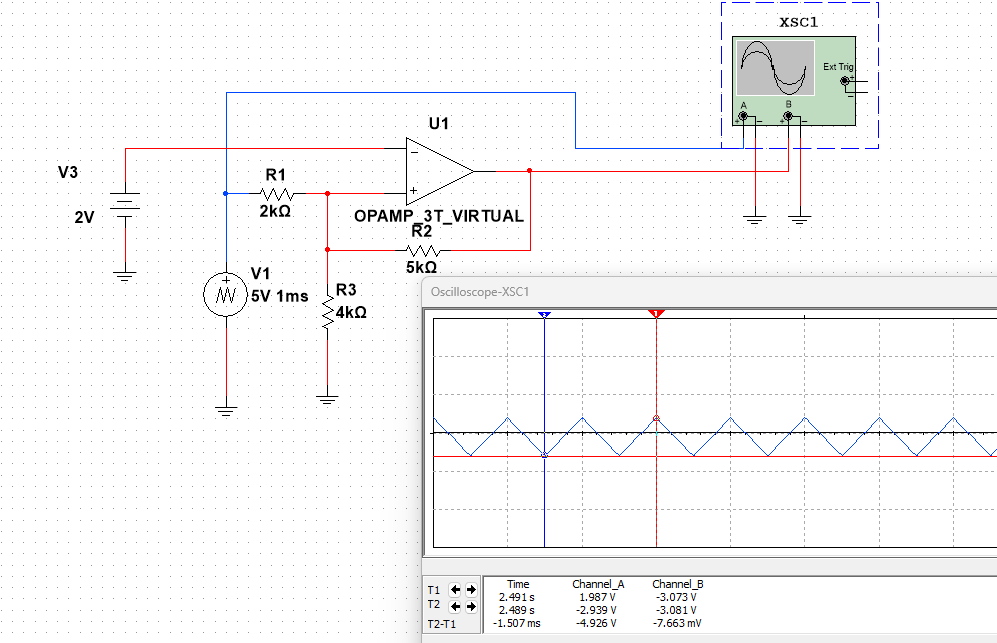
\includegraphics[width=\textwidth]{image/C12_a.png}
        \caption*{Hình a1}
    \end{subfigure}
    \hfill
    \begin{subfigure}[b]{0.48\textwidth}
        \centering
        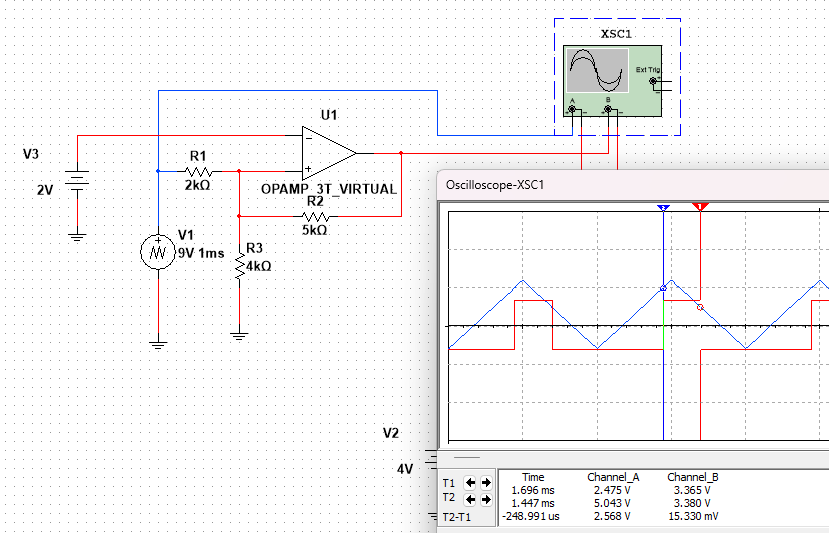
\includegraphics[width=\textwidth]{image/C12_a_1.png}
        \caption*{Hình a2}
    \end{subfigure}
\end{figure}

\textbf{Nhận xét:}\\
- Hình a1 mô phỏng $V_i$ theo đề bài với màu xanh, $V_o=-3.073V$ màu đỏ xấp xỉ -3V đúng với tính toán.\\
- Hình a2 chọn $V_i(t)$ thỏa $V_i>V_{UT}$ và $V_i<V_{LT}$ để kiểm tra lại $V_{UT}=2.475V$ và $V_{LT}=5.043V$. Đã đúng với tính toán.\\

b. Giả sử OPAMP lý tưởng:\\
Ta có:
\[
\left\{
\begin{aligned}
V^- &= V_1 \\
<<<<<<< HEAD
V^+ &= \dfrac{\dfrac{V_i}{R_1} + \dfrac{V_o}{R_2}}{\dfrac{1}{R_1} + \dfrac{1}{R_2} + \dfrac{1}{R_3}} = \dfrac{10}{19}V_i +\dfrac{4}{19}V_o
=======
V^+ &= \dfrac{\dfrac{V_i}{R_1} + \dfrac{V_0}{R_2}}{\dfrac{1}{R_1} + \dfrac{1}{R_2} + \dfrac{1}{R_3}} = \dfrac{10}{19}V_i +\dfrac{4}{19}V_o
>>>>>>> af4f750 (Done Cau 12)
\end{aligned}
\right.
\]

\[
\begin{aligned}
&\text{Giả sử }& V_o = V_{OH} &\qquad\rightarrow\qquad V^+ = \dfrac{10}{19}V_i + \dfrac{4}{19}\cdot3.3 \quad;\quad V^- = 4 \\
&\text{Để }& V_o = V_{OL} &\qquad\rightarrow\qquad V^+ < V^- \quad\rightarrow\quad \boxed{V_i<6.28V}\\
&\rightarrow& V_o = V_{OL} &\qquad\rightarrow\qquad V^+ = \dfrac{10}{19}V_i + \dfrac{4}{19}\cdot-3 \quad;\quad V^- = 4 \\
&\text{Để }& V_o = V_{OH} &\qquad\rightarrow\qquad V^+ > V^- \quad\rightarrow\quad \boxed{V_i>8.8V}\\
\end{aligned}
\]\\
Vì $V_i<6.28V \rightarrow V_o$ luôn bằng $V_{OL}=-3V$ 
\begin{figure}[H]
	\centering
	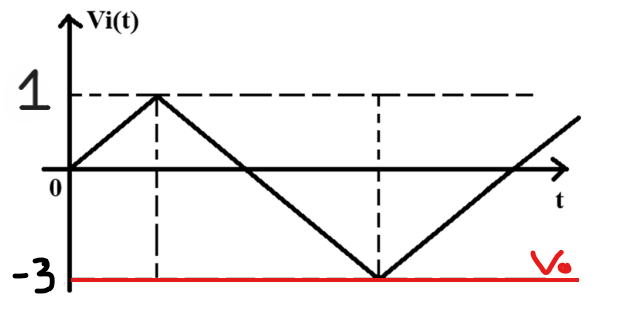
\includegraphics[scale=0.6]{image/C12_b_BT.png}
\end{figure}

\begin{figure}[H]
    \centering
    \begin{subfigure}[b]{0.45\textwidth}
        \centering
        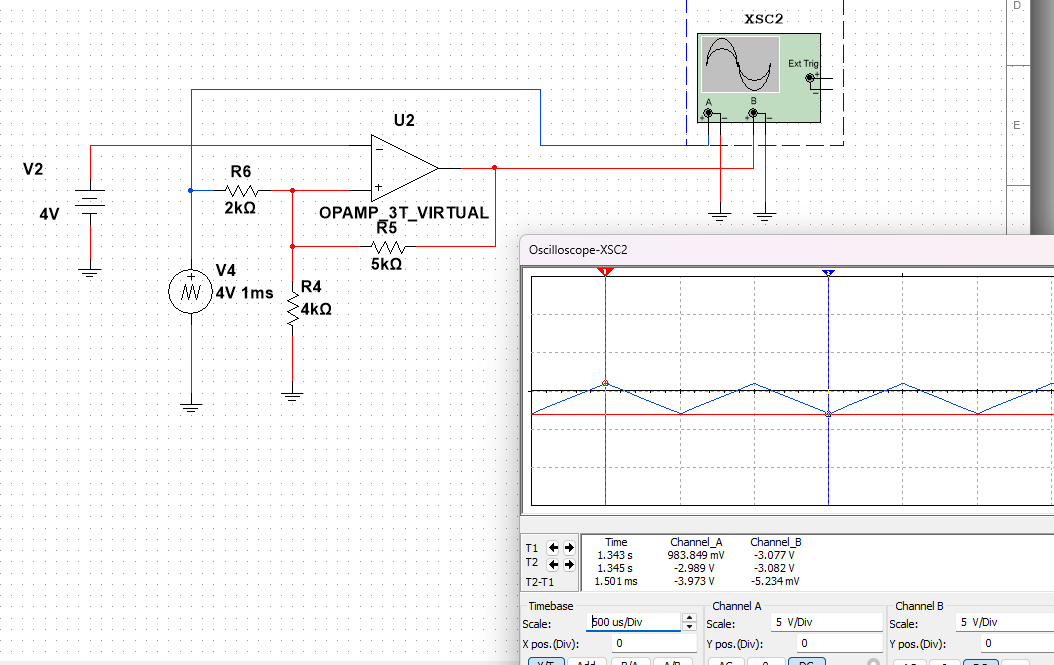
\includegraphics[width=\textwidth]{image/C12_b.png}
        \caption*{Hình b1}
    \end{subfigure}
    \hfill
    \begin{subfigure}[b]{0.5\textwidth}
        \centering
        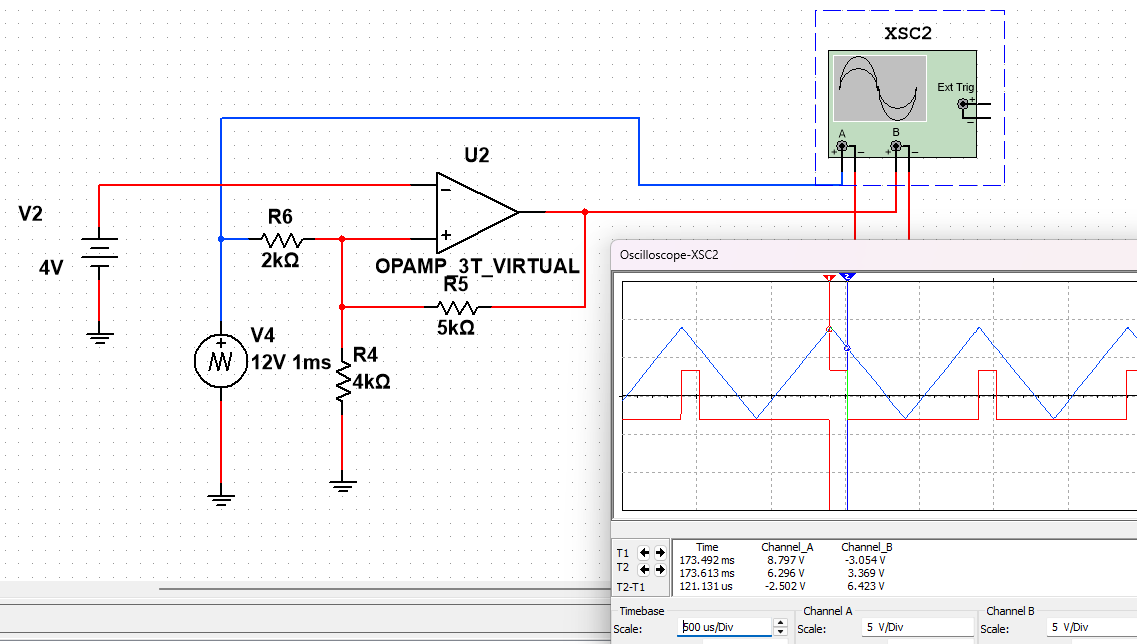
\includegraphics[width=\textwidth]{image/C12_b_1.png}
        \caption*{Hình b2}
    \end{subfigure}
\end{figure}

\textbf{Nhận xét:}\\
- Hình b1 mô phỏng $V_i$ theo đề bài với màu xanh, $V_o=-3.077V$ màu đỏ xấp xỉ -3V đúng với tính toán.\\
- Hình b2 chọn $V_i(t)$ thỏa $V_i>V_{UT}$ và $V_i<V_{LT}$ để kiểm tra lại $V_{UT}=8.797$ và $V_{LT}=6.296$. Đã đúng với tính toán.\\
